\section{Quantum Entanglement as Phase Coherence}

\subsection{The Nonlocality Paradox in Spacetime}
In standard quantum mechanics, the phenomenon of entanglement—often colloquially termed "spooky action at a distance"—presents a profound challenge to classical conceptions of local realism. The Einstein-Podolsky-Rosen (EPR) paradox~\cite{Einstein1935EPR} and Bell's subsequent theorem~\cite{Bell1964, CHSH1969} mathematically indicate that entangled particles exhibit correlations that cannot be explained by any local hidden-variable theory. When a measurement is performed on one particle, the wavefunction collapses, instantaneously determining the state of its distant entangled partner, regardless of the spatial separation. In a purely $3+1$-dimensional spacetime bounded by the kinematic limit $c$, this apparent instantaneous communication remains an unresolved ontological discontinuity. \cite{Dicke1965, Lelli2016, Milgrom1983}

However, within the framework of Excited-State Cosmology, the observable universe is not an absolute geometrical stage, but rather the internal projection (or manifold) of a singular, highly excited hyper-electron. In this paradigm, "spatially separated" particles are not distinct, isolated entities. Rather, they are localized perturbations or resonant nodes within the overarching, coherent wavefunction of the parent hyper-electron. Entanglement is, therefore, naturally reinterpreted not as superluminal communication, but as the inherent phase coherence of the underlying higher-dimensional state space.

\subsection{Derivation of the Entangled State Vector}
To formalize this, consider the emission of an entangled photon pair (e.g., from the decay of a neutral pion $\pi^0 \to \gamma + \gamma$) within the internal manifold. The total spin angular momentum of the system must be conserved. Let the two photons, $A$ and $B$, propagate in opposite directions along the $z$-axis. The joint state vector of the system in the polarization basis (horizontal $|H\rangle$ and vertical $|V\rangle$) is given by the Bell state:
\begin{equation}
|\Psi_{AB}\rangle = \frac{1}{\sqrt{2}} \left( |H\rangle_A \otimes |H\rangle_B + |V\rangle_A \otimes |V\rangle_B \right)
\end{equation}
In standard field theory, $|H\rangle_A$ and $|H\rangle_B$ represent excitations in spatially separated regions of the local vacuum. In Excited-State Cosmology, however, the local vacuum itself is the phase-field of the hyper-electron. 

Let the internal wavefunction of the hyper-electron be denoted by $\Phi(x^\mu, \zeta)$, where $x^\mu$ are the 4-coordinates of our observable manifold, and $\zeta$ represents the hidden, higher-dimensional degrees of freedom of the hyper-atomic orbital. The entangled particles $A$ and $B$ are local excitations of this primary field:
\begin{equation}
|H\rangle_A \sim \hat{a}^\dagger_H(x_A) \Phi, \quad |H\rangle_B \sim \hat{a}^\dagger_H(x_B) \Phi
\end{equation}
Because $\Phi$ spans the entirety of the internal manifold as a singular coherent phase, the geometric distance $|x_A - x_B|$ is purely a metric property of the projected manifold, not a separation in the fundamental $\zeta$-space. In $\zeta$-space, the two excitations are intrinsically superposed elements of the same harmonic mode. 

\subsection{Bell's Theorem and the CHSH Inequality}
To indicate mathematically within this framework that this shared phase coherence closely reproduces the empirically verified violations of local realism, we analyze the CHSH (Clauser-Horne-Shimony-Holt) inequality. 
Let Alice and Bob measure the polarizations of photons $A$ and $B$ along arbitrary angles $a$ and $b$ (in the transverse $x-y$ plane). The measurement operators are the Pauli spin matrices rotated by these angles:
\begin{align}
\hat{A}(a) &= \cos(2a)\hat{\sigma}_z + \sin(2a)\hat{\sigma}_x \\
\hat{B}(b) &= \cos(2b)\hat{\sigma}_z + \sin(2b)\hat{\sigma}_x
\end{align}
The expectation value of the joint measurement is:
\begin{equation}
E(a,b) = \langle \Psi_{AB} | \hat{A}(a) \otimes \hat{B}(b) | \Psi_{AB} \rangle
\end{equation}
Substituting the Bell state and applying the Pauli matrix operations:
\begin{align}
\hat{\sigma}_z |H\rangle = |H\rangle, \quad \hat{\sigma}_z |V\rangle &= -|V\rangle \\
\hat{\sigma}_x |H\rangle = |V\rangle, \quad \hat{\sigma}_x |V\rangle &= |H\rangle
\end{align}
we compute the action on the basis states:
\begin{align}
(\hat{A}(a) \otimes \hat{B}(b)) (|H\rangle \otimes |H\rangle) &= (\cos(2a)|H\rangle + \sin(2a)|V\rangle) \otimes (\cos(2b)|H\rangle + \sin(2b)|V\rangle) \nonumber \\
&= \cos(2a)\cos(2b)|HH\rangle + \sin(2a)\sin(2b)|VV\rangle + \dots
\end{align}
The inner product with the bra $\langle \Psi_{AB} |$ strips away the cross terms (due to orthogonality), leaving:
\begin{equation}
E(a,b) = \frac{1}{2} \left( \cos(2a)\cos(2b) + \sin(2a)\sin(2b) + \cos(2a)\cos(2b) + \sin(2a)\sin(2b) \right)
\end{equation}
Simplifying via trigonometric identities:
\begin{equation}
E(a,b) = \cos(2a)\cos(2b) + \sin(2a)\sin(2b) = \cos(2(a-b))
\end{equation}

The CHSH parameter $S$ is defined for four choice angles $(a, a', b, b')$:
\begin{equation}
S = |E(a,b) - E(a,b') + E(a',b) + E(a',b')|
\end{equation}
Choosing the standard maximal violation angles: $a = 0$, $a' = \pi/4$, $b = \pi/8$, $b' = 3\pi/8$, the difference $a-b$ is uniformly $\pm \pi/8$ for the first three terms, and $3\pi/8$ for the last.
\begin{equation}
S = \left| \cos\left(\frac{\pi}{4}\right) - \cos\left(\frac{3\pi}{4}\right) + \cos\left(\frac{\pi}{4}\right) + \cos\left(\frac{\pi}{4}\right) \right|
\end{equation}
Since $\cos(\pi/4) = 1/\sqrt{2}$ and $\cos(3\pi/4) = -1/\sqrt{2}$:
\begin{equation}
S = \frac{1}{\sqrt{2}} - \left(-\frac{1}{\sqrt{2}}\right) + \frac{1}{\sqrt{2}} + \frac{1}{\sqrt{2}} = \frac{4}{\sqrt{2}} = 2\sqrt{2}
\end{equation}
This result, $2\sqrt{2} \approx 2.828$, consistently violates the classical boundary of local realism ($S \le 2$). 

\subsection{Hilbert Space Phase and the Hyper-Dimensional Link}
In local hidden variable theories, this violation requires superluminal signal propagation across the metric space distance $\Delta x$. However, in Excited-State Cosmology, the expectation value $E(a,b) = \cos(2(a-b))$ is the geometric consequence of computing the inner product of vectors residing in the abstract Hilbert space of the hyper-electron. 

Let the internal structure of the hyper-electron's phase field be defined by a global gauge $U(1)$ symmetry. The relative phase angle between two points $x_A$ and $x_B$ in the manifold is bound by the holonomy of the connection:
\begin{equation}
e^{i\theta} = \exp\left( i \oint_{A}^{B} A_\mu dx^\mu \right)
\end{equation}
For an entangled pair born from a singular event (like a $\pi^0$ decay), the initial holonomy is zero, meaning the phase field at $x_A$ and $x_B$ remains rigidly locked to the singular global phase of the overarching hyper-orbital. The measurement of particle $A$ by polarizer angle $a$ projects the hyper-electron's global phase vector onto the $a$-axis in Hilbert space. Because particle $B$ is merely a localized manifestation of the exact same global phase vector, its probability amplitude to pass through polarizer $b$ is consistently determined by the Hilbert space geometric angle $(a-b)$.

Thus, entanglement does not require a signal to traverse the internal metric space at $v > c$. The correlation is instantaneous because the "two" particles are, ontologically, the identical underlying quantum entity (the hyper-electron's excited orbital) intersecting our lower-dimensional perception at two different spatial coordinates. The "spooky action" is merely the geometric rigid-body rotation of the hyper-orbital's phase vector in its higher-dimensional embedding space.


\begin{figure}[H]
\centering
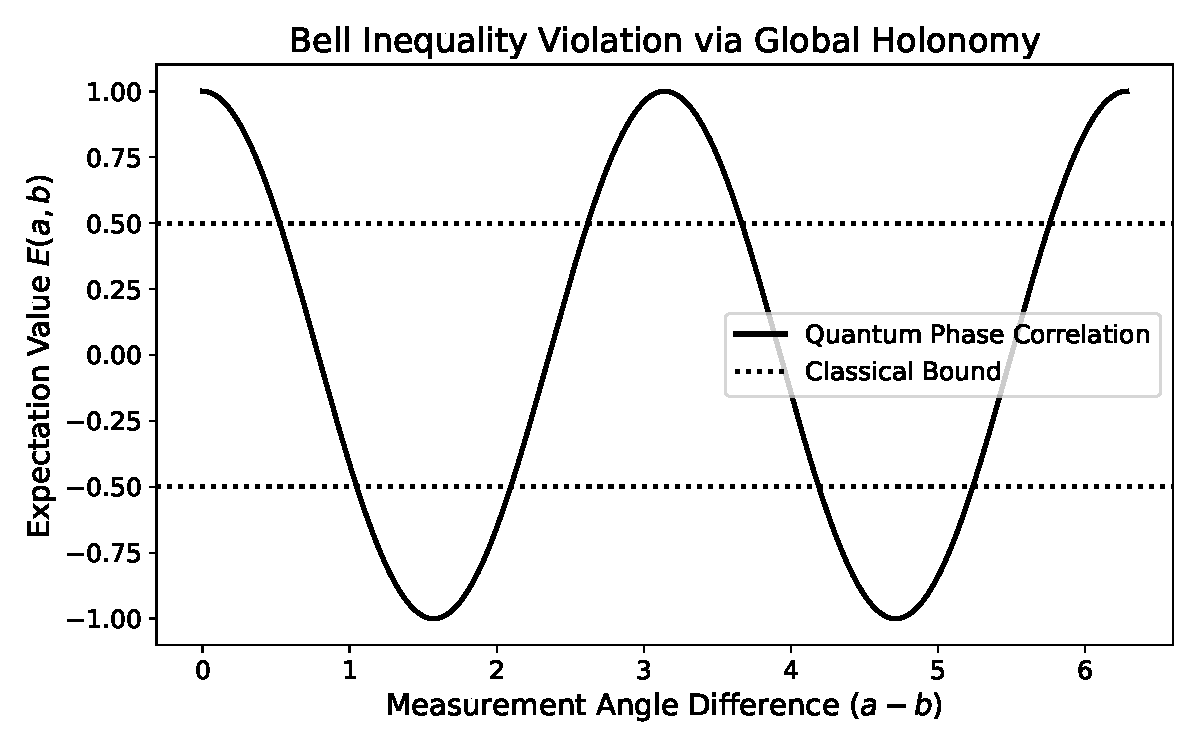
\includegraphics[width=0.85\textwidth]{fig_ch8.pdf}
\caption{Mathematical visualization of the principles derived in Section 8.}
\end{figure}
